\documentclass[]{article}

\usepackage{caption}
\usepackage{graphicx, subfig}
\usepackage{listings}
\usepackage[namelimits]{amsmath} 
\usepackage{fontspec}
\usepackage{amsmath}
\usepackage{amssymb}                      
\usepackage{mathrsfs}  
\usepackage{amsfonts}   
\setmainfont[Mapping=tex-text]{KaiTi}
\usepackage{fullpage}
\usepackage{amsthm}
\usepackage{fancyhdr}
\usepackage{algorithm}
\usepackage{algorithmic}
\usepackage{bm}
\usepackage{ctex}
\usepackage{txfonts}
\usepackage{tikz}
\usetikzlibrary{shapes.geometric, arrows}


%opening
\title{统计机器学习 课后作业6}
\author{陈劭涵 17300180049}



\newcommand{\tm}{\fontspec{Times New Roman}}


\begin{document}
	
\maketitle


\section{问题(1)}
\begin{flushleft}
解:
\end{flushleft}
$g(D,A_1)=H(D)-H(D|A_1)=0.083$, $H_{A1}(D)=(-\frac{5}{15}log\frac{5}{15}-\frac{5}{15}log\frac{5}{15}-\frac{5}{15}log\frac{5}{15})=1.58$\\\\
$\therefore g_R(D,A_1)=\frac{g(D,A_1)}{H_{A1}(D)}=0.053$\\\\
$g(D,A_2)=H(D)-H(D|A_2)=0.342$, $H_{A2}(D)=(-\frac{5}{15}log\frac{5}{15}-\frac{10}{15}log\frac{10}{15})=0.918$\\\\
$\therefore g_R(D,A_2)=\frac{g(D,A_2)}{H_{A2}(D)}=0.373$\\\\
$g(D,A_3)=H(D)-H(D|A_3)=0.420$, $H_{A3}(D)=(-\frac{6}{15}log\frac{6}{15}-\frac{9}{15}log\frac{9}{15})=0.971$\\\\
$\therefore g_R(D,A_3)=\frac{g(D,A_3)}{H_{A3}(D)}=0.433$\\\\
$g(D,A_4)=H(D)-H(D|A_4)=0.363$, $H_{A4}(D)=(-\frac{5}{15}log\frac{5}{15}-\frac{6}{15}log\frac{6}{15}-\frac{4}{15}log\frac{4}{15})=1.57$\\\\
$\therefore g_R(D,A_4)=\frac{g(D,A_4)}{H_{A4}(D)}=0.231$\\\\
因为特征$A_3$即"是否有自己的房子"的信息增益比最大,所以选择其作为根节点的特征,并将数据集$D$划分为两个子集$D_1$("是")和$D_2$("否")。由于$D_1$只有同一类的样本点,所以它成为一个叶节点,节点的标记类型为"是"\\\\
对$D_2$,从特征$A_1$,$A_2$,$A_4$中选择新的特征计算信息增益比\\\\
$g(D_2,A_1)=H(D_2)-H(D_2|A_1)=0.251$, $H_{A1}(D_2)=(-\frac{4 }{9}log\frac{4}{9}-\frac{2}{9}log\frac{2}{9}-\frac{3}{9}log\frac{3}{9})=1.53$\\\\
$\therefore g_R(D_2,A_1)=\frac{g(D_2,A_1)}{H_{A1}(D_2)}=0.164$\\\\
$g(D_2,A_2)=H(D_2)-H(D_2|A_2)=0.918$, $H_{A2}(D_2)=(-\frac{3 }{9}log\frac{3}{9}-\frac{6}{9}log\frac{6}{9})=0.918$\\\\
$\therefore g_R(D_2,A_2)=\frac{g(D_2,A_2)}{H_{A2}(D_2)}=1.000$\\\\
$g(D_2,A_4)=H(D_2)-H(D_2|A_4)=0.474$, $H_{A4}(D_2)=(-\frac{4 }{9}log\frac{4}{9}-\frac{4}{9}log\frac{4}{9}-\frac{1}{9}log\frac{1}{9})=1.39$\\\\
$\therefore g_R(D_2,A_1)=\frac{g(D_2,A_1)}{H_{A1}(D_2)}=0.341$\\\\
因为特征$A_2$即"是否有工作"的信息增益比最大,所以选择其作为根节点的特征,并将数据集$D_2$划分为两个子集$D_3$("是")和$D_4$("否")。由于$D_3$和$D_4$都只有同一类的样本点,所以它们成为最后两个叶节点,节点的标记类型分别为"是"和"否"。至此训练集中数据已经被完全分类完成\\\\
因此生成的决策树如下:\\
\begin{center}
\thispagestyle{empty}
\tikzstyle{results}=[circle ,text centered,draw=black]
\tikzstyle{decisions} =[rectangle, rounded corners,text centered, draw = black]
\tikzstyle{arrow} = [->,>=stealth]
\begin{tikzpicture}[node distance=1cm]
	\node[decisions](rootnode){是否有自己的房子};
	\node[results,below of=rootnode,yshift=-0.5cm,xshift=-2cm](rhopoint){是};
	\node[decisions,below of=rootnode,yshift=-0.5cm,xshift=2cm](touchpoint){是否有工作};
	\node[results,below of=rhopoint,yshift=-0.5cm,xshift=2cm](result4){是};
	\node[results,below of=rhopoint,yshift=-0.5cm,xshift=6cm](result5){否};
	\draw [arrow] (rootnode) -- node [left,font=\small] {是} (rhopoint);
	\draw [arrow] (rootnode) -- node [right,font=\small] {否} (touchpoint);
	\draw [arrow] (touchpoint) -- node [left,font=\small] {是} (result4);
	\draw [arrow] (touchpoint) -- node [right,font=\small] {否} (result5);
\end{tikzpicture}
\end{center}
最终叶节点的"是"和"否"表示最终的标记类别
\section{问题(2)}
\begin{flushleft}
	解:
\end{flushleft}
确定输入变量的一个切分点将输入空间划分为两个区域。随后计算所有切分点的平方误差,取那些误差最小的切分点。生成的二叉回归树如下:\\
\begin{center}
	\thispagestyle{empty}
	\tikzstyle{results}=[circle ,text centered,draw=black]
	\tikzstyle{decisions} =[rectangle, rounded corners,text centered, draw = black]
	\tikzstyle{arrow} = [->,>=stealth]
	\begin{tikzpicture}[node distance=1cm]
		\node[decisions](rootnode){[4.5, 4.75, 4.91, 5.34, 5.8, 7.05, 7.9, 8.23, 8.7, 9]};
		\node[decisions,below of=rootnode,yshift=-0.5cm,xshift=-4cm](pointl1){[4.5, 4.75, 4.91, 5.34, 5.8]};
		\node[decisions,below of=pointl1,yshift=-0.5cm,xshift=-2cm](pointl2){[4.5, 4.75, 4.91]};
		\node[decisions,below of=pointl1,yshift=-0.5cm,xshift=2cm](pointl3){[5.34,5.8]};
		\node[decisions,below of=pointl2,yshift=-0.5cm,xshift=-2cm](pointl4){[4.5]};
		\node[decisions,below of=pointl2,yshift=-0.5cm,xshift=0cm](pointl5){[4.75, 4.91]};
		\node[decisions,below of=pointl5,yshift=-0.5cm,xshift=-1cm](pointl6){[4.75]};	
		\node[decisions,below of=pointl5,yshift=-0.5cm,xshift=1cm](pointl7){[4.91]};
		\node[decisions,below of=pointl3,yshift=-0.5cm,xshift=-1cm](pointl8){[5.34]};	
		\node[decisions,below of=pointl3,yshift=-0.5cm,xshift=1cm](pointl9){[5.8]};
		\node[decisions,below of=rootnode,yshift=-0.5cm,xshift=4cm](pointr1){[7.05, 7.9 8.23, 8.7, 9]};
		\node[decisions,below of=pointr1,yshift=-0.5cm,xshift=-2cm](pointr2){[7.05, 7.9]};
		\node[decisions,below of=pointr1,yshift=-0.5cm,xshift=2cm](pointr3){[8.23. 8.7, 8.9]};
		\node[decisions,below of=pointr2,yshift=-0.5cm,xshift=-1cm](pointr4){[7.05]};
		\node[decisions,below of=pointr2,yshift=-0.5cm,xshift=1cm](pointr5){[7.9]};
		\node[decisions,below of=pointr3,yshift=-0.5cm,xshift=-1cm](pointr6){[8.23]};
		\node[decisions,below of=pointr3,yshift=-0.5cm,xshift=1cm](pointr7){[8.7, 8.9]};
		\node[decisions,below of=pointr7,yshift=-0.5cm,xshift=-1cm](pointr8){[8.7]};
		\node[decisions,below of=pointr7,yshift=-0.5cm,xshift=1cm](pointr9){[8.9]};
		\draw [arrow] (rootnode) -- node [left,font=\small] {x$\leq$ 5.8} (pointl1);
		\draw [arrow] (rootnode) -- node [right,font=\small] {x>5.8} (pointr1);
		\draw [arrow] (pointl1) -- node [left,font=\small] {x$\leq$4.91} (pointl2);
		\draw [arrow] (pointl1) -- node [right,font=\small] {x>4.91} (pointl3);
		\draw [arrow] (pointl2) -- node [left,font=\small] {x$\leq$4.5} (pointl4);
		\draw [arrow] (pointl2) -- node [right,font=\small] {x>4.5} (pointl5);
		\draw [arrow] (pointl5) -- node [left,font=\small] {x$\leq$4.75} (pointl6);
		\draw [arrow] (pointl5) -- node [right,font=\small] {x>4.75} (pointl7);
		\draw [arrow] (pointl3) -- node [left,font=\small] {x$\leq$5.34} (pointl8);
		\draw [arrow] (pointl3) -- node [right,font=\small] {x>5.34} (pointl9);
		\draw [arrow] (pointr1) -- node [left,font=\small] {x$\leq$7.9} (pointr2);
		\draw [arrow] (pointr1) -- node [right,font=\small] {x>7.9} (pointr3);
		\draw [arrow] (pointr2) -- node [left,font=\small] {x$\leq$7.05} (pointr4);
		\draw [arrow] (pointr2) -- node [right,font=\small] {x>7.05} (pointr5);
		\draw [arrow] (pointr3) -- node [left,font=\small] {x$\leq$8.23} (pointr6);
		\draw [arrow] (pointr3) -- node [right,font=\small] {x>8.23} (pointr7);
		\draw [arrow] (pointr7) -- node [left,font=\small] {x$\leq$8.7} (pointr8);
		\draw [arrow] (pointr7) -- node [right,font=\small] {x>8.7} (pointr9);
	\end{tikzpicture}
\end{center}
\section{问题(3)}
\begin{flushleft}
	解:
\end{flushleft}
若剪去$\alpha > \alpha_{i+1}$的子树$T_t$\\\\
则$g(t)=\frac{C(t)-C(T_t)}{|T_t|-1}>\alpha_i$\\\\
则$C(t)-C(T_t)>\alpha_i(|T_t|-1)$\\\\
即这棵子树划分带来的误差降低大于增加节点数带来的损失增加,所以这棵子树值得保留,剪掉的话总体误差增大\\\\
若不剪去$\alpha<\alpha_{i+1}$的子树$T_t$\\\\
则$g(t)=\frac{C(t)-C(T_t)}{|T_t|-1}<\alpha_i$\\\\
则$C(t)-C(T_t)<\alpha_i(|T_t|-1)$\\\\
即这课子树划分带来的误差降低小于增加节点数带来的损失增加,所以这棵子树不值得保留,留着的话会是总体误差增大\\\\
所以使用$\alpha\in[\alpha_i,alpha_{i+1}]$剪枝得到的子树$T_i$是区间内的最优子树\\\\
\section{问题(4) 实战题}
\begin{flushleft}
	解:
\end{flushleft}
一.
\begin{lstlisting}[language=R]
data=read.csv("D:/大数据学院文件资料/2020秋课程/机器学习/assignment/homework6/simudata.csv")
\end{lstlisting}
随后我读了数据说明并了解了各自变量的含义\\\\
二.
\begin{lstlisting}[language=R]
boxplot(billnum~black,data=data,col=c("dodgerblue","coral2"),
border=c("dimgray","dimgrey"),
main='交易笔数~是否违约的箱线图',names=c("不违约","违约"),
xlab="是否违约",ylab="交易笔数",plot=T)

boxplot(meanpay~black,data=data,col=c("dodgerblue","coral2"),
border=c("dimgray","dimgrey"),
main='所有行为均值~是否违约的箱线图',names=c("不违约","违约"),
xlab="是否违约",ylab="所有行为均值",plot=T)
\end{lstlisting}
箱线图如下:\\\\
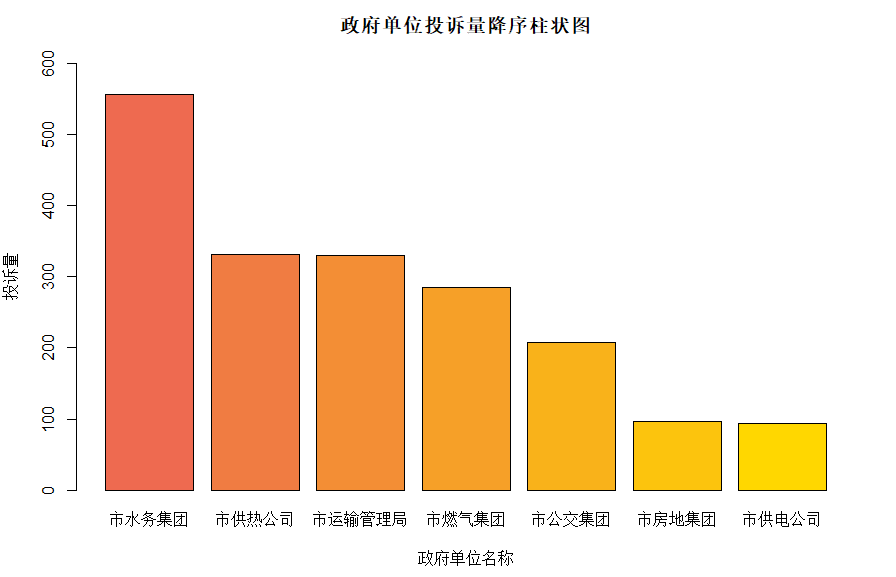
\includegraphics[width=.9\textwidth]{D:/大数据学院文件资料/2020秋课程/机器学习/homework/hw6/1.png}\\\\
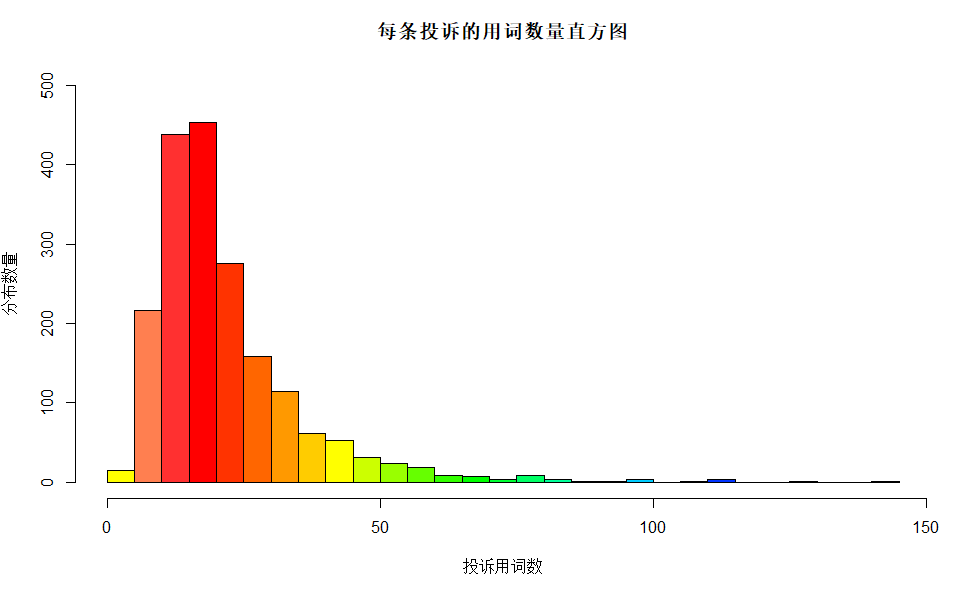
\includegraphics[width=.9\textwidth]{D:/大数据学院文件资料/2020秋课程/机器学习/homework/hw6/2.png}\\\\
解读:\\
1、从第一个箱线图中我们可以看到,违约用户的交易笔数分布相对于不违约用户更少,说明交易笔数少的用户更有可能违约;\\
2、从第二个箱线图中我们可以看到,违约用户的所有行为均值分布相对于不违约用户更少,说明所有行为均值更少的用户更有可能违约\\\\
三.
\begin{lstlisting}[language=R]
set.seed(1234)
split=sample(2,nrow(data),replace=T,prob=c(0.7,0.3))
train=data[split==1,]
test=data[split==2,]

library("rpart")
model=rpart(black~.,data=train,method="class")

pred=predict(model,test,type="class")
pred
(sum(pred==test$black))/nrow(test)

library("pROC")

roc(test$black,as.numeric(pred)-1,plot=TRUE,main="测试集ROC曲线",xlab = "FPR", ylab = "TPR",
print.thres=TRUE,print.auc=TRUE,legacy.axes=TRUE,grid=c(0.2,0.2),
grid.col="dimgray",auc.polygon=TRUE,max.auc.polygon=TRUE,auc.polygon.col="darkslategray1",max.auc.polygon.col="deepskyblue")
\end{lstlisting}
预测准确度以及ROC曲线、AUC值如下:
\begin{lstlisting}[language=R]
> (sum(pred==test$black))/nrow(test)
[1] 0.6967905
\end{lstlisting}
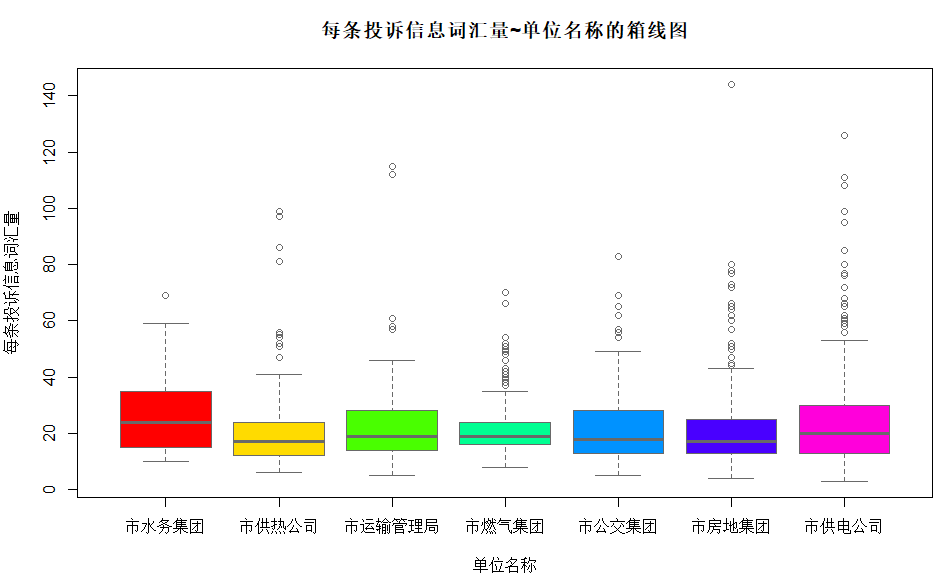
\includegraphics[width=1.\textwidth]{D:/大数据学院文件资料/2020秋课程/机器学习/homework/hw6/3.png}\\\\
AUC值为0.594\\\\
四.
\begin{lstlisting}[language=R]
library(rpart.plot)
rpart.plot(model)
\end{lstlisting}
决策树图形如下:\\\\
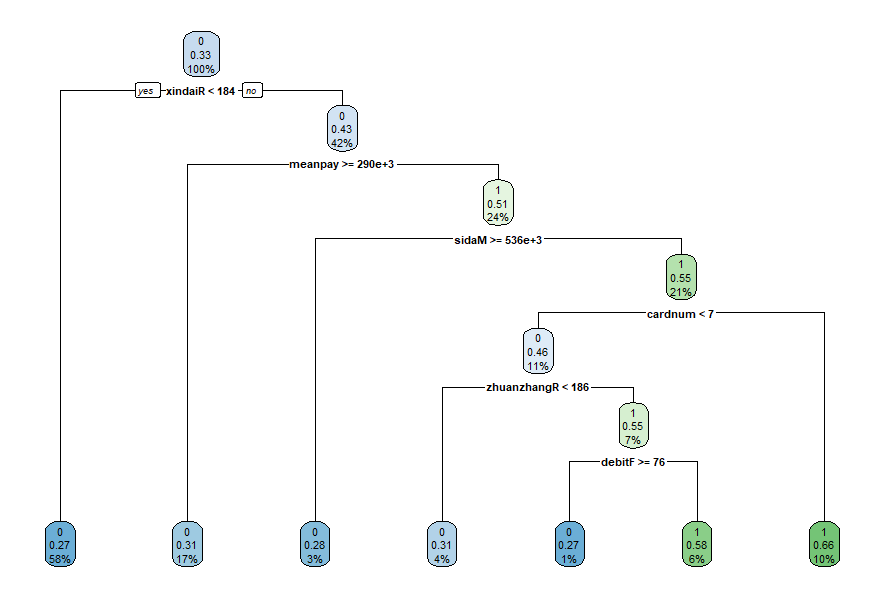
\includegraphics[width=1.\textwidth]{D:/大数据学院文件资料/2020秋课程/机器学习/homework/hw6/4.png}\\\\
解读:\\
1、从决策树模型中我们可以看到,模型认为最具有区分度的特征是xindaiR是否小于184。说明用户的近期贷款情况对于模型识别用户是否违约非常具有参考性。此外meanpay是否大于290e+3也是其次的但非常重要的区分特征,所有行为均值越大的用户越不可能违约;\\
2、cardnum,zhuanzhangR,debitF也是具有一定区分度的特征。说明用户的银行卡数,近期转账,借记类M也是具有一定参考价值的变量。而根据决策树模型,数据集中的其他自变量相对来说没有表现出特别强的说明能力,所以没有在决策树中出现
\end{document}
